\begin{figure}[H]
    \centering
    % Hình 1 bên trái
    \begin{subfigure}[b]{0.45\textwidth} % Độ rộng chiếm 45% chiều rộng văn bản
        \centering
        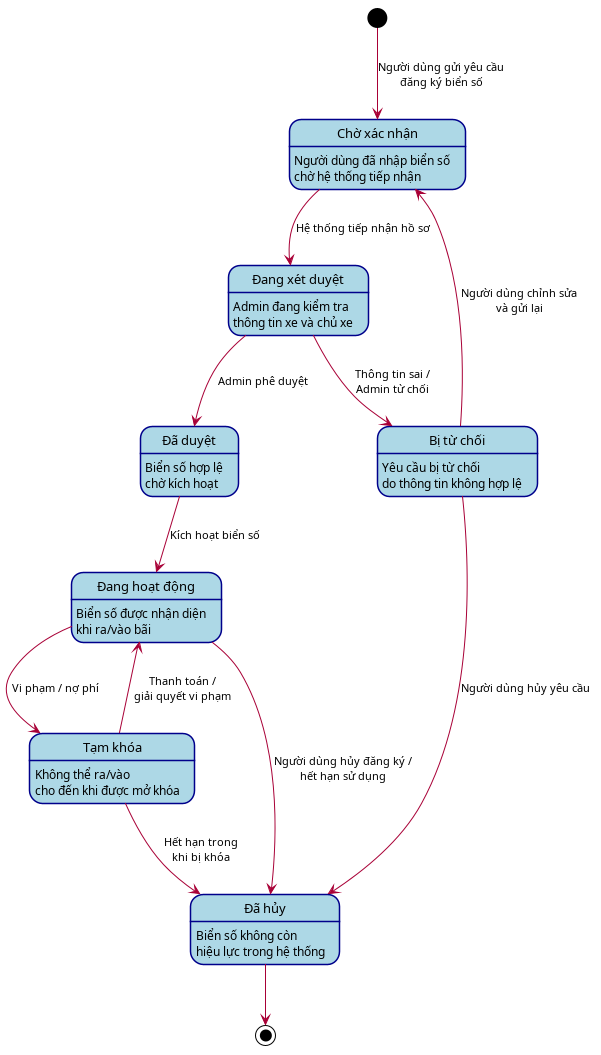
\includegraphics[width=\linewidth]{pictures/statechart1.png}
        \caption{State Chart --- Phiên đăng ký biển số}
        \label{fig:statechart1}
    \end{subfigure}
    \hfill % Khoảng trống linh hoạt giữa hai hình
    % Hình 2 bên phải
    \begin{subfigure}[b]{0.45\textwidth} % Độ rộng chiếm 45% chiều rộng văn bản
        \centering
        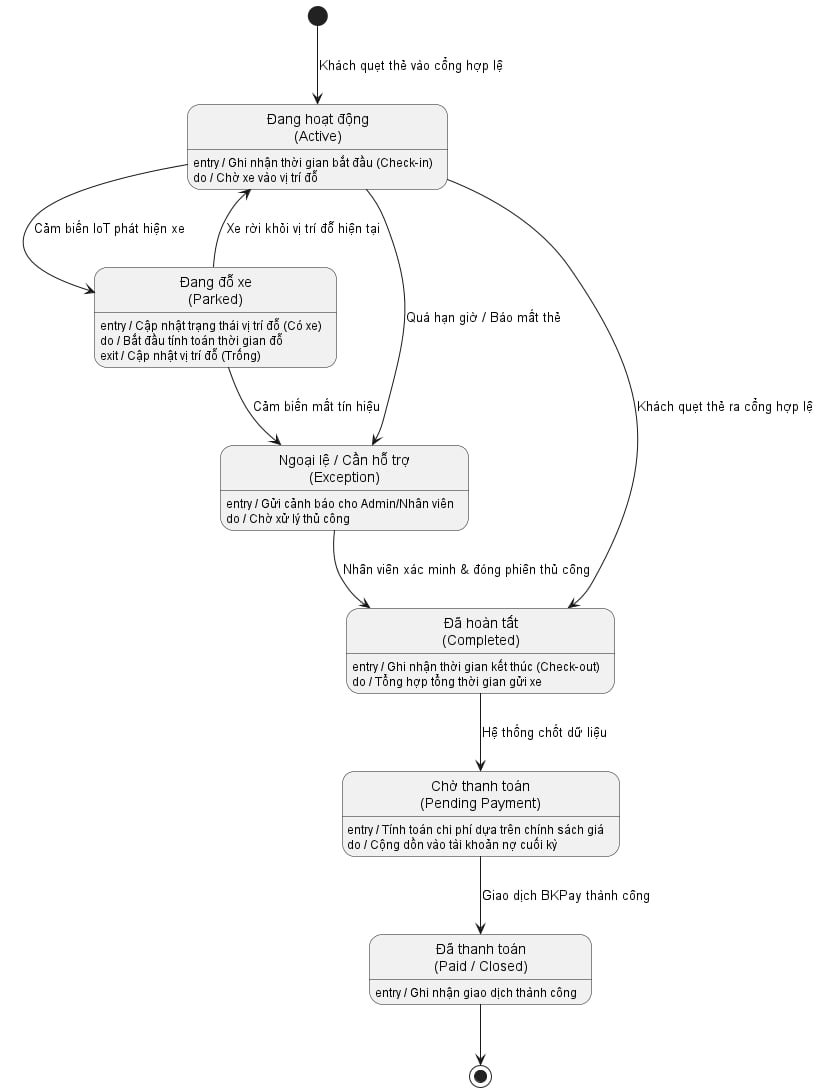
\includegraphics[width=\linewidth]{pictures/statechart2.png} % Điều chỉnh width một chút để cân đối hơn nếu cần
        \caption{State Chart --- Phiên gửi xe}
        \label{fig:statechart2}
    \end{subfigure}
    
    % Chú thích chung cho cả cụm hình (tùy chọn)
    \caption{Các State Chart trong hệ thống}
    \label{fig:both_statecharts}
\end{figure}

Hệ thống quản lý bãi xe thông minh được thiết kế dựa trên hai biểu đồ trạng thái chính, phân chia rõ ràng giữa khâu quản lý dữ liệu và khâu vận hành thực tế. Biểu đồ đầu tiên thể hiện quy trình quản lý vòng đời của một biển số xe trong hệ thống, bao quát các bước từ lúc người dùng nộp yêu cầu đăng ký, chờ quản trị viên xét duyệt để kích hoạt, cho đến các trạng thái phát sinh trong quá trình sử dụng như tạm khóa do vi phạm hoặc nợ phí, và cuối cùng là hủy bỏ dịch vụ. Song song đó, biểu đồ thứ hai tập trung vào luồng hoạt động cụ thể của một lượt gửi xe. Quy trình này mô tả chi tiết trình tự các sự kiện diễn ra từ thời điểm khách hàng quẹt thẻ vào cổng, hệ thống nhận diện xe thông qua cảm biến tại vị trí đỗ, cho đến lúc khách quẹt thẻ ra và hoàn tất thủ tục thanh toán để rời bãi.
\newpage